\chapter{Genomic Meta-Feature Guided Regularized Regression for Survival Outcome}
\label{cha:xtunecox}

\section{Abstract}
In building predictive models for genomic studies, regularized regression is a common technique as the number of genomic features is much larger than the number of samples. The application of sparse regularized regression performs feature selection while doing prediction. Associated with genomic features, such as gene expression, genetic variation, DNA methylation, there are plenty of meta-features. Some examples are functional gene sets, gene ontology annotations, knowledge of past studies. Existing method is to model genomic features on phenotypic outcomes, and post hoc analysis with meta-features, like gene set enrichment analysis. However, incorporating meta-features into modeling process can potentially improve the quality of both prediction performance and feature selection. 

In this paper, we extend the approach of \cite{zeng2021incorporating} to survival outcome. The method incorporates genomic meta-features to guide the regularized Cox regression, so that each of the genomic features has its own customized penalty parameter, as opposed to one common penalty parameter for all features. With highly informative meta-features, significant features become more important/being penalized less, unrelated features become less important/heavily penalized, thereby achieving improved feature selection. The prediction performance is also improved with the extra meta-feature information. We show the benefits of the method by simulations and applications in genomic studies. Model optimization algorithm involves empirical Bayes estimation of penalty parameters, and a majorization-minimization procedure. 

\section{Introduction}
Predicting a phenotypic outcome based on genomic features is a highly active research area, with the increasing need in personalized health care to achieve the best outcome for individual patients. A common technique for genomic predictive modeling is regularized regression. As the number of genomic features is typically large, thousands to millions, linear models like regression are better suited. Because the data pattern is most likely linear where each feature contribute a little or none effect to the outcome. When number of features is larger than the number of samples, which is usually the case for genomics study, regularization needs to be introduced so that the model can be fit. Sparse regularized regression is a popular choice, as it not only shrinks the regression coefficients to make the model simpler, it also shrink some of the coefficients with little effects on the outcome to exactly zero, thereby performing feature selection. Typical examples are the lasso \citep{tibshirani1996regression} and the elastic net \citep{zou2005regularization}. While they have similar mechanics, there is a major difference. If some of the features among which the correlations with each other are high, the lasso tends to select one of them, while the elastic net tends to select most of them and share the lasso value equally. Ridge regression \citep{hoerl1970ridge} is another regularization technique to cope with high dimension and collinearity of data. However, it only shrinks the coefficients, not to zero, hence does not produce interpretable model. 

Genomic features may have their own characteristics: grouping effect and ordering. Extensions of the lasso deal with such situations. The group lasso \citep{yuan2006model} takes in the grouping information, shrinking coefficients by group. All the coefficients in one group are either zero or nonzero. Sparse group lasso \citep{simon2013sparse} further allows sparsity within group. The fused lasso deals with the ordering situation, with the addition of $L_1$ terms for the differences of neighbouring coefficients, which allows sparsity in their differences. The above extended regularization methods take into account characteristics of features, which are essentially features of the features if they are put in a data set. We call these underlying characteristics of features "meta-features" here and after. There are plenty of such meta-features in genomics. For example, functional gene sets like hallmark \citep{liberzon2015molecular}, gene ontology pathways like reactome \citep{jassal2020reactome} work as grouping effect; summary statistics like p-values and regression coefficients from meta-analyses work as ordering effect (p-values and regression coefficients indicate the importance of each feature). The meta-features are actual data matrices, where the samples/rows represent original features, and the columns represent meta-features. However, none of the above regularization approaches systematically utilize the meta-feature information. The group lasso assumes features are in different groups mutually exclusive. Features in multiple groups at the same time does not meet the assumption. The fused lasso takes the ordering of the features into account, but when provided with concrete information like p-values indicating exactly how important each feature are, it cannot incorporate such information. 

One way of utilizing the meta-features is modeling with original features, and performing gene set enrichment analysis \citep{subramanian2005gene} post hoc. However, incorporating meta-features into modeling process can potentially improve both prediction performance and the quality of feature selection. Weaver et al. (reference) and Shen et al. (reference) incorporate the meta-features in a hierarchical modeling setup. The outcomes are regressed on original features, assuming quantitative outcome, 
$$ \bm{Y} = \bm{X\beta} + \bm{\varepsilon} $$ 
where $\bm{Y}$ is the length $n$ outcome vector, $\bm{X}$ is the $n \times p$ data matrix, $\bm{\beta}$ is the length $p$ feature coefficient vector to be estimated in the model. Then the feature coefficients $\bm{\beta}$ are regressed on meta-features,
$$ \bm{\beta} = \bm{Z\alpha} + \bm{\gamma} $$
where $\bm{Z}$ is the $p \times q$ meta-feature matrix, $\bm{\alpha}$ is coefficients vector for meta-features. To integrate both level of features into modeling process, an objective function is formed as below 
$$ \min_{\bm{\beta, \alpha}} \frac{1}{2n} \|\bm{Y}-\bm{X \beta} \|_2^2 + \frac{\lambda_1}{2} \|\bm{\beta} - \bm{Z \alpha} \|_2^2 + \lambda_2 \|\bm{\alpha}\|_1 $$
The original feature data $\bm{X}$ and meta-feature data $\bm{Z}$ are fitted through two least squares. The additional $L_1$ term of meta-feature coefficients $\bm{\alpha}$ is to control model complexity and meta-feature selection. This integration method incorporates meta-features linearly, emphasizing on meta-feature selection. It was shown to improve the prediction performance considerably with high quality meta-features. \cite{zeng2021incorporating} developed another method for integrating meta-features $\bm{Z}$ for quantitative and binary outcomes, in a non-linear way, such that each of the original features has its own customized penalty parameter, as opposed to one common penalty parameter for all features. The customized penalty parameters potentially allow more accurate feature selection. In this paper, we extend this approach to survival outcomes. 

\section{Methods}
\subsection{Model setup and notations}
Starting with the survival model setup, let the outcome data be $(\bm{y, \delta})$ where $\bm{y}=(y_1,y_2,\dots,y_n)$ is observed time, $\delta=(\delta_1,\delta_2,\dots,\delta_2)$ is censoring status. If $\delta_i = 1 (i=1,2,\dots,n)$, event happened, $y_i$ is event time; if $\delta_i=0$, event did not happen in experimental period, $y_i$ is censoring time. There are $p$ features for the n instances/samples, data matrix $\bm{X}$ with dimension $n\times p$ stores the feature values, i.e., $\bm{x}_i$ is a vector of feature values for instance $i$ $(x_{i1},x_{i2},\dots,x_{ip})$. Associated with the features, there are q meta-features. A $p\times q$ matrix $\bm{Z}$ stores the meta-feature values for the $p$ original features, i.e., $\bm{z}_j (j=1,2,\dots,p)$ is a vector of meta-feature values for feature $j$ $(z_{j1},z_{j2},\dots,z_{jq})$. The common choice of regression method is Cox's proportional hazards model \citep{cox1972regression}. It assumes hazard functions are proportional at the same time point, which allows model fitting without knowing explicit form of baseline hazard function, and only depends on the order in which events occur, not on the exact time of occurrence. To illustrate, let $t_1<t_2<\dots<t_l<\dots<t_m$ be the the unique event times arranged in increasing order, and $D_l=\{i:\delta_i=1,y_i=t_l\}$ is the set of instances experienced event at time $t_l$. Let $\bm{\beta}$ be a length $p$ vector for the feature regression coefficients. The partial likelihood function, $L(\bm{\beta})$, takes the form 
\begin{displaymath}
L(\bm{\beta}) = \prod_{l=1}^{m} \frac{e^{\sum_{i\in D_l}\bm{x}_i^T\bm{\beta}}}{(\sum_{i\in R_l} e^{\bm{x}_i^T\bm{\beta}})^{d_l}}
\end{displaymath}
where $R_l=\{i: y_i\geq t_l\}$ is the risk set at event time $t_l$, i.e., the set of all instances who have not experienced the event and are uncensored just prior to time $t_l$; $d_l=|D_l|$ is the number of events at time $t_l$. $L(\bm{\beta})$ is Breslow's adjustment of partial likelihood \citep{breslow1972contribution}. It deals with ties in each event time ($d_l>1$: more than one instance experienced event at a particular event time). When there are no ties ($d_l=1$), $L(\bm{\beta})$ automatically reduces to Cox's partial likelihood. We can see that neither hazard functions nor times are involved in the function, only the order of event times matters. 

We add regularization to Cox regression to control model complexity. Denote the log of partial likelihood as $\ell(\bm{\beta})$,
\begin{equation} \label{eq1}
    \min_{\bm{\beta}\in \mathbb{R}^p} \left\{-\ell(\bm{\beta}) + \lambda\left[\frac{1}{2}(1-c)\|\bm{\beta}\|_2^2 + c\|\bm{\beta}\|_1\right]\right\}.
\end{equation}
The regularization function covers lasso, elastic net, ridge penalties, i.e., $c=1$ represents the lasso, $c=0$ represents ridge, and $0<c<1$ represents the elastic net. When $0<c\leq1$, it is sparse regularization which shrink some coefficients to exactly zero, producing interpretale model. The regularization has a universal penalty parameter $\lambda$ for all the features. This ignores underlying characteristics of features assuming each of them are equally important by applying the same amount of penalty. Our idea is to incorporate informative meta-features which might indicate the importance of the original features, giving each of them a unique penalty parameter $\lambda_j$. To incorporate meta-features to $\lambda_j$, first form a linear combination of $\bm{z_j}$ for feature $j$, $\bm{\alpha}$ is the weight vector of length $q$; then give it a non-linear function by expenentiating it
\begin{equation} \label{eq2}
\begin{aligned}
    &\min_{\bm{\beta}\in \mathbb{R}^p} \left\{-\ell(\bm{\beta}) + \sum_{j=1}^p \lambda_j\left[\frac{1}{2}(1-c)\beta_j^2 + c|\beta_j|\right]\right\}, \\
    &\lambda_j = e^{\bm{z_j}^T \bm{\alpha}}.
\end{aligned}
\end{equation}

\subsection{Model fitting}
The standard regularized Cox proportional hazards model, equation \eqref{eq1}, is fitted with pathwise coordinate descent \citep{simon2011regularization}. As the universal penalty parameter $\lambda$ is a hyper-parameter, the algorithm constructs a $\lambda$ path to tune via cross-validation. The proposed model, equation \eqref{eq2}, has $p$ $\lambda$'s decided by weights $\bm{\alpha}$, $\bm{\lambda} = (\lambda_1,\lambda_2,\dots,\lambda_p) = e^{\bm{Z\alpha}}$, it is impossible to tune them. Instead, we estimate the weights $\bm{\alpha}$ first to get the values of $\bm{\lambda}$. With known $\bm{\lambda}$, we can fit the model via coordinate descent.

\subsubsection{Empirical Bayes estimation of hyperparameter} \label{laplace}
To estimate $\bm{\alpha}$, we need to form an objective function. Since the regularized regression has a natural Bayesian  interpretation, we apply empirical Bayes estimation of hyper-parameters in random effects model, which is maximizing marginal likelihood in terms of hyper-parameter $\bm{\alpha}$ obtained by integrating out random effects $\bm{\beta}$. Based on the Bayesian elsatic net \citep{li2010bayesian}, equation \eqref{eq2} has the interpretation
\begin{align}
    &f(\bm{Y}|\bm{\beta}; \bm{X}) = L(\bm{\beta}) \label{eq3}, \\
    &\pi(\beta_j; \bm{\alpha}) \propto exp\left\{ -\lambda_j\left[\frac{1}{2}(1-c)\beta_j^2 + c|\beta_j|\right] \right\}. \label{eq4}
\end{align}
With the likelihood \eqref{eq3} and prior distribution \eqref{eq4}, we construct the joint distribution of $\bm{Y}$ and $\bm{\beta}$, and integrate out $\bm{\beta}$, so to get the marginal likelihood of $\bm{Y}$,
\begin{align*}
\ln f(\bm{Y};\bm{\alpha}) &= \int_{\bm{\beta}\in\mathbb{R}^p} \ln f(\bm{Y}, \bm{\beta};\bm{\alpha}) d\bm{\beta} \\
&= \int_{\bm{\beta}\in\mathbb{R}^p} \left[\ln f(\bm{Y}|\bm{\beta};\bm{X})+\ln \pi(\bm{\beta};\bm{\alpha})\right]d\bm{\beta} \\
&= \int_{\bm{\beta}\in\mathbb{R}^p} \left\{ \sum_{l=1}^{m}\left[\sum_{i\in D_l}\bm{x}_i^T\bm{\beta}-d_l\ln(\sum_{i\in R_l} e^{\bm{x}_i^T\bm{\beta}})\right] - \sum_{j=1}^{p} \lambda_j\left[\frac{1}{2}(1-c)\beta_j^2 + c|\beta_j|\right]+ \text{const} \right\} d\bm{\beta}
\end{align*} 
This integral does not have a closed form expression because the elastic net prior is not a conjugate prior for the likelihood. We propose two approximation procedures: first approximate the elastic net prior to a normal prior, then apply Laplace approximation. To approximate the elastic net prior, we follow Zeng et al. (2021) (reference),  
\begin{equation}
    \pi(\beta_j; \bm{\alpha}) = N(0, \frac{2}{2\lambda_j(1-c)+c^2\lambda_j^2}). \label{eq5}
\end{equation}
Equation \eqref{eq5} gives a similar variance to that of the elastic net prior. The joint distribution, $\ln f(\bm{Y}, \bm{\beta};\bm{\alpha})$, then takes the form 
\begin{equation} \label{eq6}
\begin{aligned}
    &\ln f(\bm{Y}, \bm{\beta};\bm{\alpha}) = \sum_{l=1}^{m}\left[\sum_{i\in D_l}\bm{x}_i^T\bm{\beta}-d_l\ln(\sum_{i\in R_l} e^{\bm{x}_i^T\bm{\beta}})\right] - \sum_{j=1}^{p} \frac{1}{2}v_j\beta_j^2 + \text{const}, \\
    &v_j = \frac{2\lambda_j(1-c)+c^2\lambda_j^2}{2}.
\end{aligned}
\end{equation}
This is essentially a ridge regularized Cox regression with customized penalty vector. 
For Laplace approximation of the marginal likelihood/model evidence, we elaborate the details. Consider a Taylor series of $\ln f(\bm{Y}, \bm{\beta};\bm{\alpha})$ at the stationary point $\widetilde{\bm{\beta}}$, where $\nabla \ln f(\bm{Y}, \widetilde{\bm{\beta}};\bm{\alpha})=0$,
$$ \ln f(\bm{Y}, \bm{\beta};\bm{\alpha}) \approx \ln f(\bm{Y}, \widetilde{\bm{\beta}};\bm{\alpha}) - \frac{1}{2}(\bm{\beta}-\widetilde{\bm{\beta}})^T\bm{H}(\bm{\beta}-\widetilde{\bm{\beta}}). $$
$\widetilde{\bm{\beta}}$ is the solution of a ridge regularized Cox regression as already stated, it can be computed using \textbf{R} language \emph{glmnet} package \citep{simon2011regularization}, with known $\bm{\alpha}$. $\bm{H}$ is the Hessian matrix,
\begin{align*}
    \bm{H} &= - \nabla\nabla \ln f(\bm{Y}, \bm{\beta};\bm{\alpha})|_{\bm{\beta}=\widetilde{\bm{\beta}}} \\
    & \approx \bm{X}^T\bm{W}\bm{X} + \bm{V}
\end{align*}
where $\bm{V} = \text{diag}[\bm{v}]=\text{diag}[v_1,\dots,v_p]$, $\bm{W}$ is a diagonal matrix with elements 
$$ \bm{W}_{ii} = \sum_{l\in C_i}\frac{d_le^{\bm{x}_i^T\bm{\beta}}}{\sum_{k\in R_l}e^{\bm{x}_k^T\bm{\beta}}} - \sum_{l\in C_i}\frac{d_l(e^{\bm{x}_i^T\bm{\beta}})^2}{(\sum_{k\in R_l}e^{\bm{x}_k^T\bm{\beta}})^2}. $$ 
The Hessian is an approximation because $W$ is in fact a full matrix with high computational cost. We only use diagonal elements to speed up computation without much loss of accuracy. For greater details, refer to Shen et al. (2021) (reference).
Now that we see $f(\bm{Y}, \bm{\beta};\bm{\alpha})$'s Taylor approximation has a multivariate normal form with mean $\widetilde{\bm{\beta}}$, variance $\bm{H}^{-1}$, integrating out $\bm{\beta}$ returns the normalizing constant.
\begin{equation} \label{eq7}
\begin{aligned}
    -\ln{f(\bm{Y};\bm{\alpha})} &\approx -\ln f(\bm{Y}|\widetilde{\bm{\beta}};\bm{X}) - \ln \pi(\widetilde{\bm{\beta}};\bm{\alpha}) - \frac{p}{2}\ln{2\pi} + \frac{1}{2}\ln{|\bm{H}|} \\
    &= -\ln{|\bm{V}|} + \widetilde{\bm{\beta}}^T\bm{V}\widetilde{\bm{\beta}} + \ln{|\bm{H}|} + \text{const}
\end{aligned}
\end{equation}
The approximate negative log marginal likelihood, equation \eqref{eq7}, is the objective function we are going to minimize with respect to $\bm{\alpha}$.

\subsubsection{Objective function optimization} \label{DCA}
The objective function, equation \eqref{eq7}, is nonconvex. In particular, it can be decomposed as difference of two convex functions. $g(\bm{\alpha}):=-\ln{|\bm{V}|} + \widetilde{\beta_j}^T\bm{V}\widetilde{\beta_j}$ is convex in $\bm{\alpha}$, whereas $h(\bm{\alpha}):=\ln{|\bm{H}|}$ is concave. This makes it a proper candidate to apply difference of convex functions algorithm (DCA) \citep{le2015dc}. The principle idea of DCA is to approximate the nonconvex objective function by a sequence of convex ones: at each iteration of the sequence, approximate the concave part by its affine majorization, i.e., the supporting hyperplane obtained by calculating its gradient, or subgradients if not differentiable, and minimize the resulting convex approximation. Note that it is also an application of majorization-minimization algorithm \citep{hunter2004tutorial}. The affine approximation of the concave part is the majorization step, which forms a surface lying above the objective function, and is tangent to it, i.e, at the current estimation of the target parameter, the majorization equals to the objective function. This ensures the majorization is a tight upperbound for the objective. Minimizing the convex upperbound is the minimization step. The DCA algorithm for the marginal likelihood, $-\ln{f(\bm{Y};\bm{\alpha})}$:
\begin{enumerate}
    \item Initialize $\bm{\alpha}$ with $\widetilde{\bm{\alpha}} \in \mathbb{R}^q$.
    \item Majorization: 
    \begin{itemize}
        \item calculate the gradient at current estimation $\widetilde{\bm{\alpha}}$,
    $$\bm{\theta}= \nabla_{\bm{v}} \ln{|\bm{H}|} = \text{diag}[\bm{H}^{-1}]$$ 
        \item form the convex upperbound,
        \begin{align*}
        u(\bm{\alpha})&=g(\bm{\alpha})+ h(\widetilde{\bm{\alpha}}) + \bm{\theta}^T(\bm{v}-\widetilde{\bm{v}}) \\
        &=-\ln{|\bm{V}|} + \widetilde{\bm{\beta}}^T\bm{V}\widetilde{\bm{\beta}}+\bm{\theta}^T\bm{v}+\text{const}
        \end{align*}
    \end{itemize}
    \item Minimization: $\hat{\bm{\alpha}}=\underset{\bm{\alpha}}{\operatorname{\argmin}} \left\{u(\bm{\alpha})\right\}$.
    \item Set $\widetilde{\bm{\alpha}} = \hat{\bm{\alpha}}$.
    \item Repeat step 2-4 until convergence of $\hat{\bm{\alpha}}$.
\end{enumerate}
The minimization of $u(\bm{\alpha})$ can be processed with standard first order method like gradient descent, or second order method like Newton-Raphson. We show the gradient and Hessian here,
\begin{align*}
    &\nabla_{\bm{\alpha}} u(\bm{\alpha}) = \bm{Z}^T\left[(-\frac{1}{\bm{v}}+\widetilde{\bm{\beta}}^2+\bm{\theta})((1-c)\bm{\lambda}+c^2\bm{\lambda}^2)\right],\\
    &\nabla\nabla_{\bm{\alpha}} u(\bm{\alpha}) = \bm{Z}^T \text{diag}\left[\frac{\bm{\lambda}^2}{\bm{v}^2}(1-c+c^2\bm{\lambda})^2+(-\frac{1}{\bm{v}}+\widetilde{\bm{\beta}}^2+\bm{\theta})\bm{\lambda}(1-c+2c^2\bm{\lambda})\right]\bm{Z}.
\end{align*}

\subsection{Summary}
We incorporate the meta-features into the penalty parameter of regularized Cox proportional hazards model, as a log-linear function, to give each feature a unique penalty parameter depending on the meta-features. We then apply Bayesian interpretation of regularized regression to obtain the marginal likelihood function, as the objective function to optimize with respect to the introduced meta-feature weights $\bm{\alpha}$, thereby estimating the customized penalty parameter vector $\bm{\lambda}$. The nonconvex objective function can be decomposed to a difference of two convex functions, which can be solved with difference of convex functions algorithm. With estimated $\bm{\alpha}$, we can plug values of penalty parameters into the regularized Cox regression. The model fitting procedure is
\begin{enumerate}
    \item Initialize $\bm{\alpha}$ with $\widetilde{\bm{\alpha}}$.
    \item Repeat, until convergence of $\hat{\bm{\alpha}}$.
    \begin{enumerate}
        \item Laplace approximation of marginal likelihood with known $\widetilde{\bm{\alpha}}$, section \ref{laplace},
        \begin{itemize}
            \item Approximate the elastic net prior with a normal prior, equation \eqref{eq6},
            \item Calculate $\widetilde{\bm{\beta}}$ and $\bm{H}$.
        \end{itemize}
        \item Optimize Laplace approximation of marginal likelihood, equation \eqref{eq7}, get solution $\hat{\bm{\alpha}}$, with DCA described in section \ref{DCA}.
        \item Set $\widetilde{\bm{\alpha}} = \hat{\bm{\alpha}}$.
    \end{enumerate}
    \item Calculate customized penalty vector $\bm{\lambda}=e^{\bm{Z}\hat{\bm{\alpha}}}$.
    \item Fit regularized Cox regression, equation \eqref{eq2}, with $\bm{\lambda}$.
    
\end{enumerate}

\section{Simulations}
\subsection{Simulation methods}
In this section, we perform simulations to evaluate the model performance. The purpose of the simulation is to compare prediction, feature selection between our proposed model and standard regularized Cox regression. We generate meta-feature data $\bm{Z}$ from independent Bernoulli variables, with probability 0.1. This is to simulate biological pathway/functional gene set meta-features. Each pathway contains a group of genes, 1 indicates the gene being in the pathway group, 0 otherwise. Meta-feature weights $\bm{\alpha}$ are set to be fixed, values are from -1 to 1 equally spaced. We then can generate $\bm{\beta}$ from its normal prior distribution with mean 0, variance computed from $\bm{\alpha, Z}$, equation \eqref{eq5}. Note that we want the underlying model to be sparse, so we keep the top 20\% of the $\bm{\beta}$ elements with largest absolute values, and set the remaining to be 0. In this step, we can control the informativeness of the meta-features. Once $\bm{\beta}$ are generated, meta-features are fully informative to the model. We randomly change some of the rows of $\bm{Z}$ to opposite values (0 to 1, 1 to 0) so that the proportion of rows modified indicates the informativeness of meta-features, i.e., 10\% of the rows modified shows high informativeness while 90\% of the rows modified indicates low informativeness. Data matrix $\bm{X}$ are distributed as a multivariate normal with an autoregressive correlation structure, $\bm{\Sigma}_{ij} = \rho^{|i-j|}$, set $\rho=0.5$. Survival times are generated based on inverse probability integral transform,   
\begin{displaymath}
t = H_0^{-1}\left(-\ln(U)e^{-\bm{\beta}^T\bm{x}}\right)
\end{displaymath}
where $U\sim \text{uniform}[0,1]$, $H_0(t) = (t/5)^8$ is the baseline cumulative hazard function with Weibull distribution. Censoring time is from an exponential distribution, $c\sim \text{exp}(0.1)$. The distribution parameter values set for Weibull and exponential are to produce survival times range from 0 to 20, and a fixed ratio of events to censoring. We then add a normal noise to survival times to fix the model underlying predictive ability at concordance measure \citep{harrell1982evaluating} 0.8, by controlling the standard deviation of the noise. The survival time outcome is set to be the minimum of survival and censoring time, $y=\text{min}(t,c)$. And it is said to be censored $\delta=0$ if $c<t$, the observation loses follow up before event happens. 

For each simulation, we generate data as described above. We fit standard elastic net regularized Cox regression without external meta-features $\bm{Z}$, and also fit our proposed model with meta-features. Elastic net regression is tuned with 5-fold cross validation, while the proposed model does not require penalty parameter tuning as it is estimated during model fitting procedure. We then compare the prediction performance between the two models on simulated test set. The simulation steps are performed with 100 replicates. 

We run a series of experiments varying one key parameter while keeping the others fixed. The base case parameters are sample size $n=100$, feature size $p=200$, meta-feature size $q=10$, meta-feature $\bm{Z}$ informativeness: 5\% of features (rows of $\bm{Z}$) has been modified to have incorrect values. This is a high informativeness level. 4 experiments are conducted by varying one parameter at a time.
\begin{enumerate}
    \item Meta-feature informativeness level from high to low, proportion of rows of $\bm{Z}$ modified 5\%, 15\%, 30\%.
    \item Feature size, $p=200, 600, 1000$.
    \item Sample size, $n=100, 200, 300$.
    \item Meta-feature size, $q=10, 20, 30$.
\end{enumerate}
In experiment 1, we also examined quality of feature selection by both models, to evaluate how informativeness of meta-features influences model interpretation.

\subsection{Simulation results}
Figure \ref{fig:sim21} shows the results of 4 simulation experiments. The horizontal dashed line in each panel represents the population/theoretical C-index, achievable with infinite samples of training data. It is provided as a reference for each parameter setting. The performance of meta-feature guided elastic net Cox model (denoted as `meta' in the figure) is compared to that of a standard elastic net Cox model. 

In experiment 1, there are consistent improvements in prediction performances as long as the meta-features are informative. The higher the informativeness of meta-features, the more improvements gained in prediction performance over the standard elastic net model. In the figure, the difference of test C-index between the two models increases with the informativeness of meta-features. 

Experiment 2 illustrates model performances with respect to feature size. Larger number of features relative to sample size makes it harder for both models to predict, as both models' test C-indexes are way below the theoretical C-index, 0.8, when feature size is 600 and 1000. However, the meta-feature model consistently performs better than standard elastic net model.

Experiment 3 evaluates a similar situation as experiment 2, instead of varying feature size, it varies sample size while keeping 200 features. As sample size gets larger, i.e, feature size to sample size ratio becomes smaller, both models perform better, and meta-feature guided elastic net consistently performs better than the standard elastic net. Furthermore, larger sample size produces more stable prediction metrics (smaller variance of test C-index). 

As the size of meta-features increases (experiment 4), the prediction performance improvement over the standard elastic net becomes smaller. This indicates the meta-feature guided model's inability to handle higher dimension of meta-features.  

In terms of the quality of feature selection, we define accurate selection as follow: features with non-zero simulated coefficients are estimated with non-zero values; features with zero simulated coefficients are estimated as zero. In Figure \ref{fig:sim22}, we compared feature selection accuracy among meta-feature guided elastic net model, standard elastic net model with the $\lambda$ value that gives maximum cross-validated C-index (denoted as `enet.min'), and with the $\lambda$ value that gives the most regularized model such that the cross-validated C-index is within one standard error of the maximum (denoted as `enet.1se'), in experiment 1, where the informativeness of meta-features varies. The `1se' elastic net model is sparser (less nonzero coefficients) than the `min' elastic net model. The proposed meta-feature guided elastic model again outperforms both standard elastic net models in feature selection accuracy. Moreover, the selection is more stable with meta-features compared to either of the standard elastic net models. Note that the selection accuracy of the `min' elastic net model is highly unstable, since its model is more dense than the `1se' elastic net, and the meta-feature guided model.
\begin{figure}
    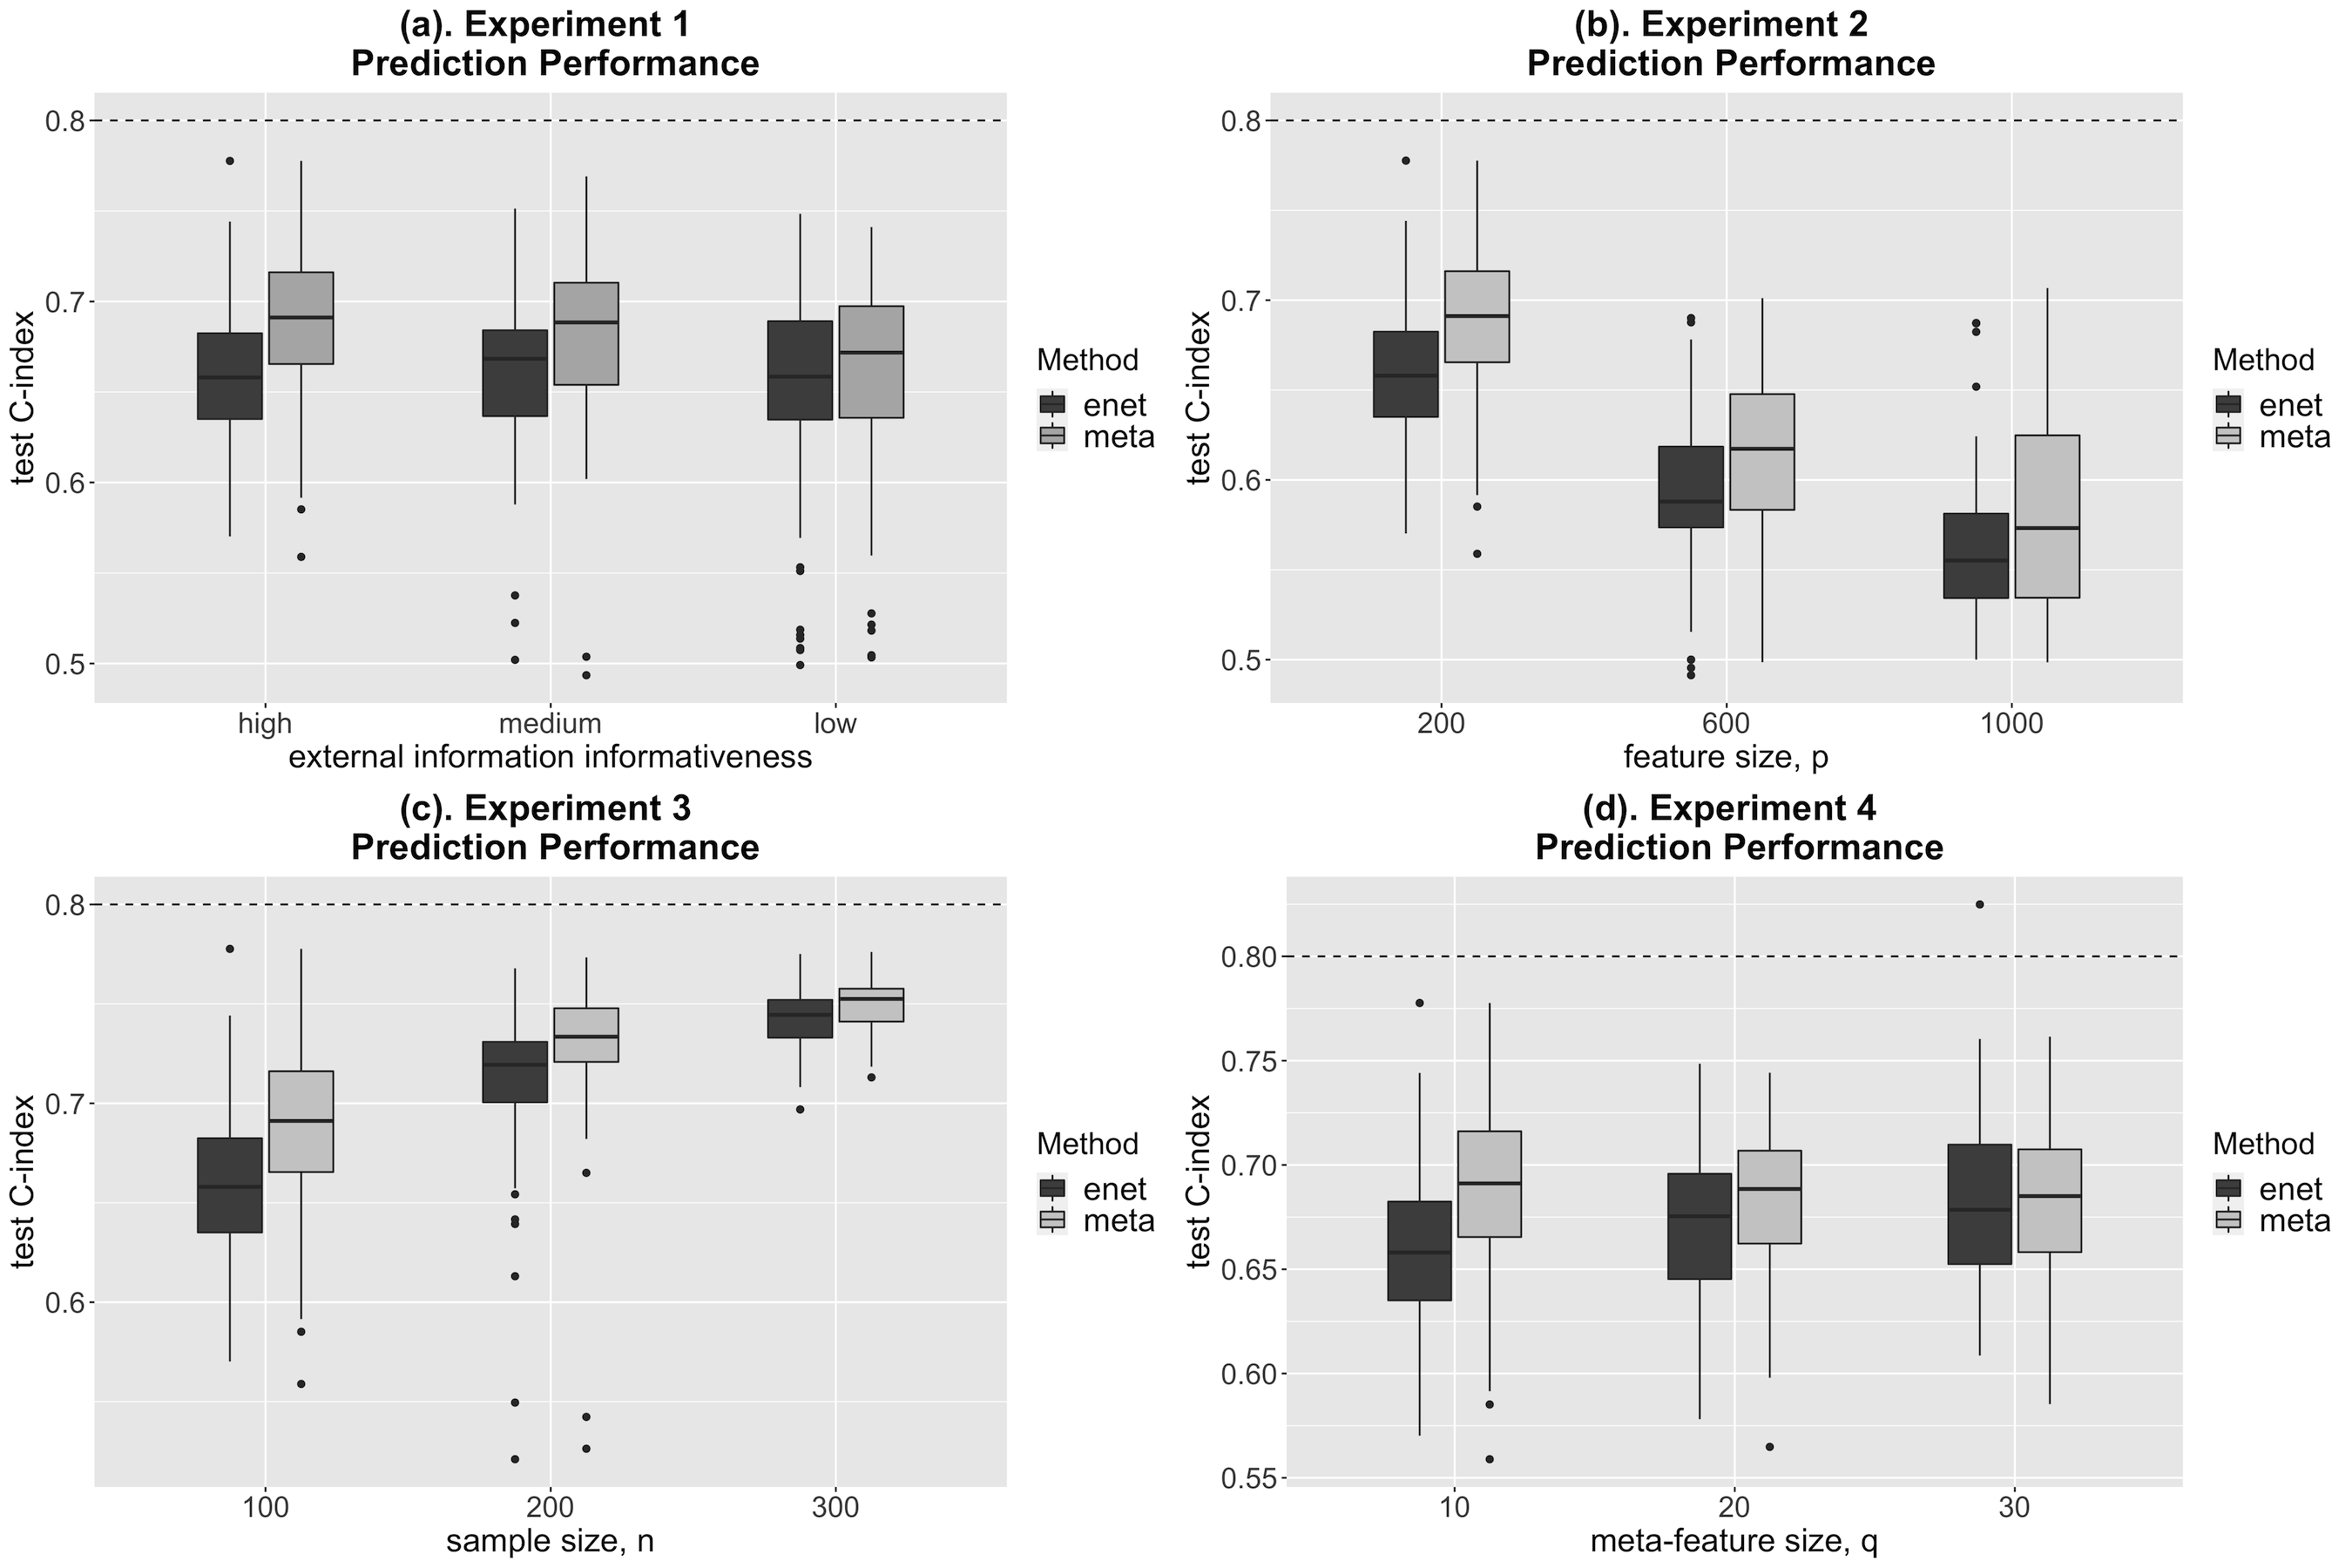
\includegraphics[width=\textwidth]{sim21}
    \caption{Simulation: prediction performance }
    \label{fig:sim21}
\end{figure} 

\begin{figure}
    \centering
    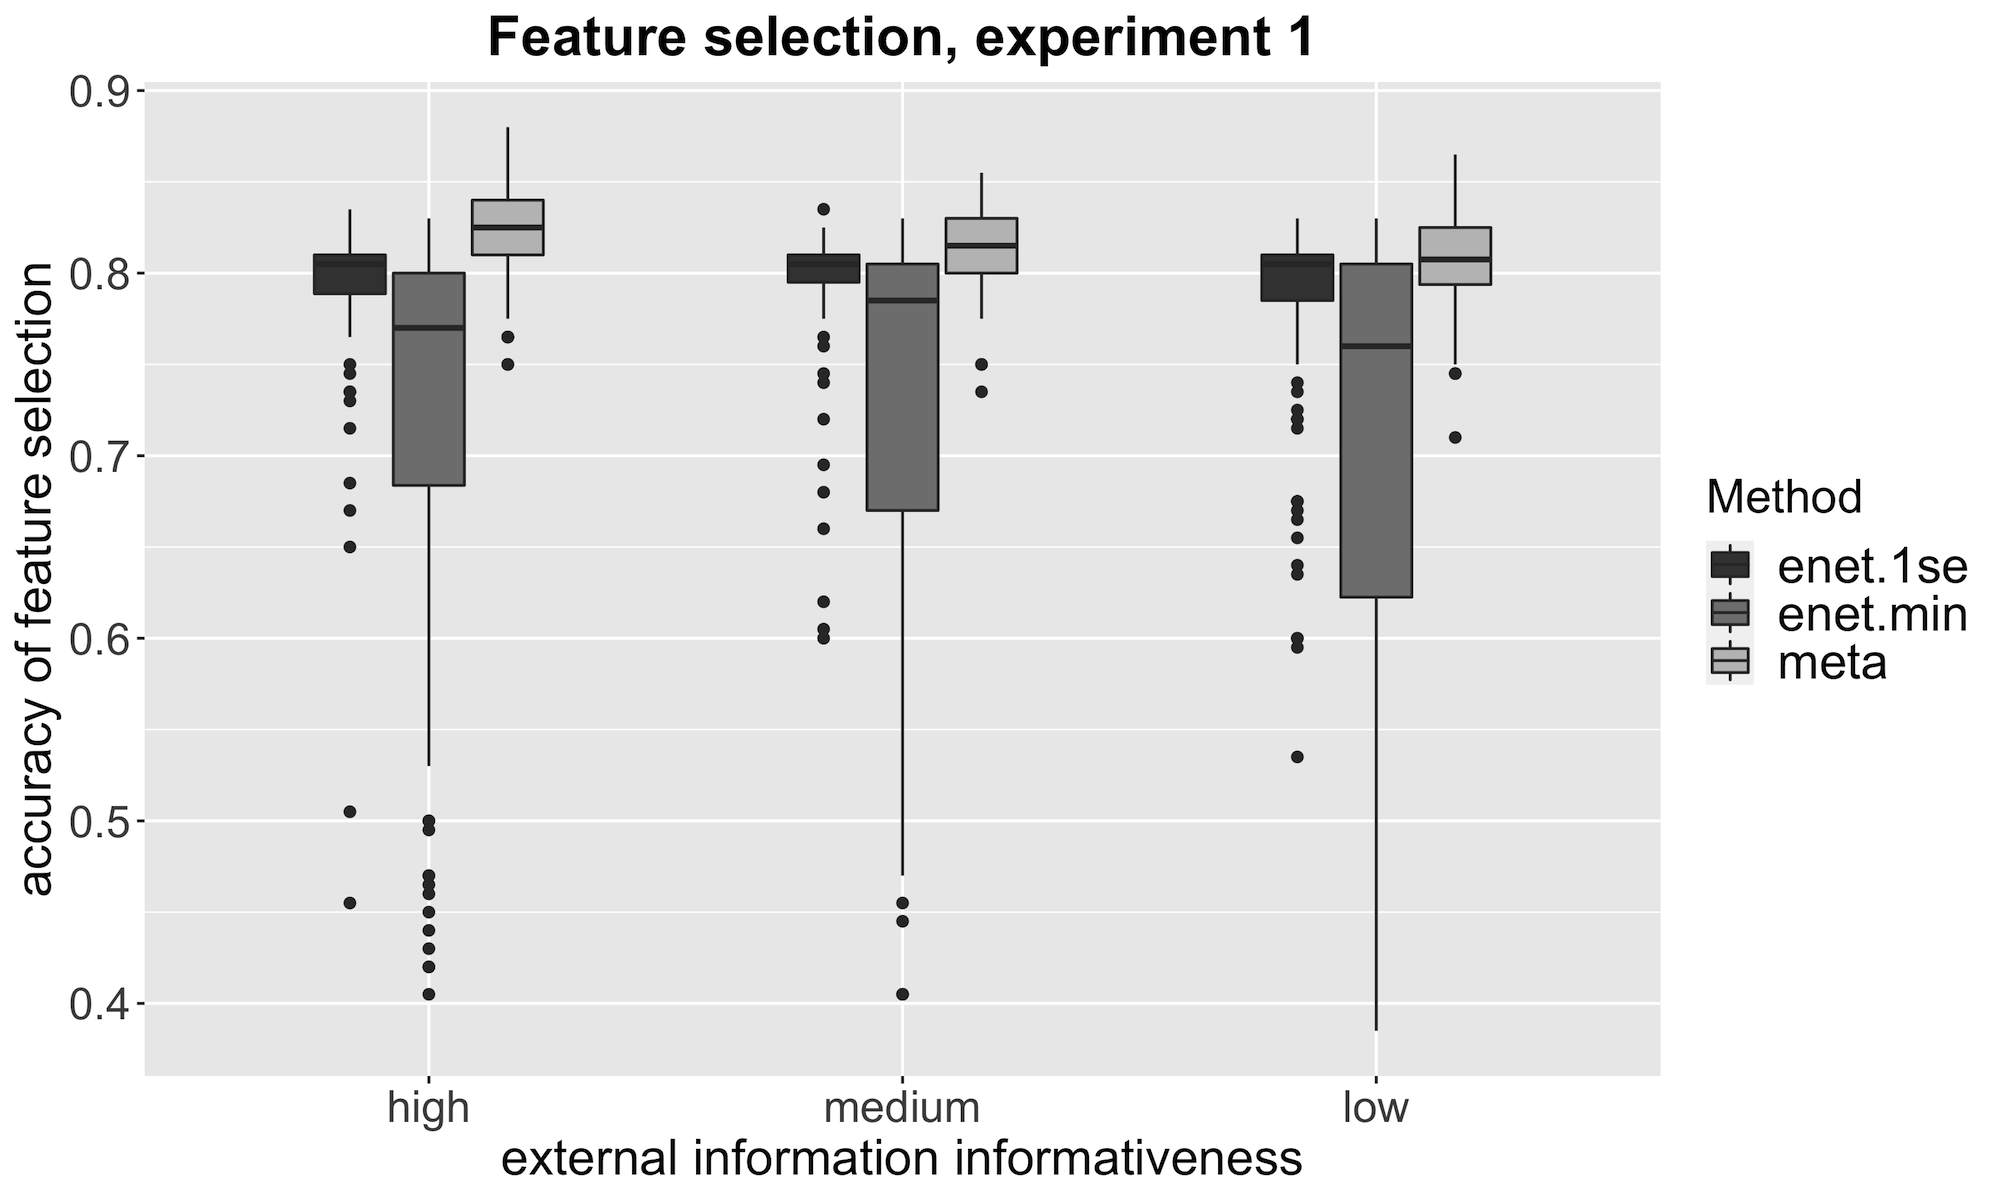
\includegraphics[scale=0.7]{sim22}
    \caption[Simulation: feature selection]{Simulation: feature selection. `enet.min' is the standard elastic net model with the $\lambda$ value that gives maximum cross-validated C-index; `enet.1se' is the elastic net model with the $\lambda$ value that gives the most regularized model such that the cross-validated C-index is within one standard error of the maximum.}
    \label{fig:sim22}
\end{figure}

\section{Applications}
We also applied the proposed meta-feature model to a melanoma data set to predict overall survival in patients treated with PD-1 immune checkpoint blockade. The programmed death 1 pathway (PD-1) is an immune-regulatory mechanism used by cancer to hide from the immune system. Antagonistic antibodies to PD-1 pathway and its ligands, programmed death ligand 1 (PD-L1), demonstrate high clinical benefit rates and tolerability. Immune checkpoint blockades such as Nivolumab, pembrolizumab are anti-PD-1 antibodies showing improved overall survival for the treatment of advanced melanoma. However, less than 40\% of the patients respond to the treatments \citep{moreno2015anti}. Therefore, predicting treatment outcomes, identifying predictive signals are of great interest to appropriately select patients most likely to benefit from anti-PD-1 treatments. We explored transcriptomes and clinical data using our model to illustrate prediction performance and predictive signal selection.

The dataset combined 3 clinical studies in which RNA-sequencing were applied to patients treated with anti-PD1 antibodies, \cite{gide2019distinct, riaz2017tumor, hugo2016genomic}. The gene expression values are normalized toward all sample average in each study as the control, so that they are comparable to one another across features within a sample and comparable to one another across samples. There are 16010 gene in common across 3 studies, and combined 117 subjects. The clinical variables being considered are age, gender, and tumor response. We build predictive models in terms of overall survival, based on transcriptomics and clinical variables. Since the subjects are all treated with anti-PD1 antibodies, the transcriptomic features selected by the model are predictive signals for treatment efficacy or resistance. We selected meta-features from molecular signature database, hallmark gene sets \citep{liberzon2015molecular}. 13 gene sets are enriched \citep{subramanian2005gene} to have false positive rates less than 0.25 (Table \ref{table3.1}). An indicator matrix is formed to illustrate whether each of the 16010 genes belong to one of the 13 hallmark gene sets ($\bm{Z}$). 

We compared prediction and feature selection performance between meta-feature guided elastic net model and standard elastic net model. The data is split into training and test set (3:1). Standard elastic net is trained using 5-fold cross validation, while meta-feature model is trained with estimated hyperparameters. The test concordance index is 0.7340 for the elastic net, and 0.7609 for our meta-feature guided model. As for feature selection, the meta-feature model, which selects 4 transcriptomes (GPAA1, COX6C, VPS28, PLCB4), is sparser, as opposed to 11 features selected in the elastic net model. 
\begin{table}[tbh]
    \centering
    \def\arraystretch{1.3}
    \begin{tabular}{|c|c|}
    \hline
     \bf Hallmark meta-feature & \bf Estimated $\bm{\alpha}$ \\
     \specialrule{.1em}{.05em}{.05em}
     Interferon gamma response & -0.0102  \\ \hline
     Allograft rejection & 0.1570  \\ \hline
     Interferon alpha response & -0.0314 \\ \hline
     IL6 JAK STAT3 signaling & 0.1131 \\ \hline
     Inflammatory response & 0.0744 \\ \hline
     Complement & 0.1577 \\ \hline
     TNFA signaling via NFKB & 0.1180 \\ \hline
     IL2 STAT5 signaling & 0.1613 \\ \hline
     Bile acid metabolism & 0.0876 \\ \hline
     Kras signaling down & 0.2338 \\ \hline
     Xenobiotic metabolism & 0.2598 \\ \hline
     Apoptosis & 0.2557 \\ \hline
     Kras signaling up & 0.2737 \\ \hline
    \end{tabular}
    \caption[List of hallmark meta-features and their respective estimated weight]{List of hallmark meta-features and their respective estimated weight $\bm{\alpha}$. Weights are estimated from empirical Bayes hyperparameter tuning.}
    \label{table3.1}
\end{table}

\section{Discussion}
In this paper, we extended to survival outcome a customized regularization model guided by genomic meta-features. This model has unique penalty parameters for each of the features instead of one common penalty parameter for all the features in standard regularized regression. This differential penalty amount allows each feature to be of different importance to the outcome of interest, guided by their underlying characteristics. With the feature characteristics highly informative, the important features will be penalized less (less shrinkage, less likely to be 0), and the not so important features will be penalized heavier (heavier shrinkage, more likely to be 0, excluded from the model), so that achieving better feature selection. For the range of simulation results and data application in anti-PD1 immunotherapy predictive modeling, the customized regularization model showed benefits in prediction performance, and the selected model tend to be sparser (less features selected). Note that we do need the external meta-feature data to be informative with less noise meta-features, because the proposed model does not predicts as well with the increase in dimension of meta-features. Therefore, we need prior knowledge to select meta-features. However, the proposed model is a systematic way to incorporate external meta-features that will most likely provide insight on how to further modeling the data.

In the setting of incorporating meta-feature into regularized regression, we have developed 2 methods to systematically utilize them in modeling process. The method in this paper integrates meta-features in a non-linear way. It allows the meta-features to decide the importance of each feature by defining the penalty parameters as a non-linear function of meta-features. As opposed to this method, Weaver et al. [] and Shen et al. [] integrates meta-features linearly, which implemented in R package `xrnet'. The fundamental difference between the 2 methods is that `xrnet' models meta-features through the mean of $\bm{\beta}$, while the proposed model in this paper models meta-features through the variance of $\bm{\beta}$. As they both have underlying hierarchical structure to model features and meta-features, `xrnet' assumes meta-features are a linear regression of feature regression coefficients, $\bm{\beta} \sim N(\bm{Z\alpha}, \tau\bm{I})$, therefore, the mean of $\bm{\beta}$ is determined by $\bm{Z\alpha}$. In the customized regularization model, $\bm{\beta}$ has an approximated prior $N(0, \frac{2}{2\lambda_j(1-c)+c^2\lambda_j^2})$, we can see the variance is determined by meta-features. In practice, it is hard to tell which one is in favor to another. Depending on the application at hand, one would want to try both as different data has different dynamics. 

Our proposed model applied empirical Bayes to estimate penalty parameters for each feature, which uses Laplace approximation to obtain the marginal likelihood. Laplace approximation works well when sample size is relatively large. We see in simulation experiment 2, while our model shows prediction benefits in all feature sizes, there is a decreasing trend of benefits over standard elastic net Cox regression, which might caused by the drop of quality in Laplace approximation when sample size is too small relative to feature size. We did not fully address how well Laplace approximation is in the modeling process, and how it will affect the model performance. We need to be careful when applying the model to ultra high dimensional data. 

We have mentioned that the proposed customized regularization model does not handle higher dimension of meta-features very well. This is because no regularization is applied to meta-feature weights $\bm{\alpha}$, or control its complexity in some form. As a result, the model fitting algorithm is not able to deal with large number of meta-features efficiently and stably. Careful selection of meta-features is needed rather than fitting all external information at hand. In simulation experiment 4, the prediction improvement decrease as we increase the number of meta-features. With continuous development of gene annotation database, more summary statistics from meta-analyses, future work in regularizing meta-features is a potential improvement of the model to expand its ability of handling high dimensional meta-feature data.
